\documentclass[landscape,a0paper,fontscale=0.30]{baposter}

\usepackage[vlined]{algorithm2e}
\usepackage{times}
\usepackage{calc}
\usepackage{url}
\usepackage{graphicx}
\usepackage{amsmath}
\usepackage{amssymb}
\usepackage{pifont}
\usepackage{relsize}
\usepackage{multirow}
\usepackage{booktabs}
\usepackage{natbib}
\usepackage{tcolorbox}
\usepackage{wrapfig}

\usepackage{graphicx}
\usepackage{multicol}
\usepackage[T1]{fontenc}
\usepackage{tgadventor}
\usepackage{ae}
\usepackage{enumitem}

\usepackage{colortbl}
\usepackage{xcolor}
\graphicspath{{images/}{imgs/}}

\bibliographystyle{abbrv}
\setlength{\bibsep}{0.1pt}
\newcommand{\cmark}{{\color{green}\ding{51}}}%
\newcommand{\xmark}{{\color{red}\ding{55}}}%
\definecolor{tumblue}{rgb}{0, 0.2, 0.9}
\definecolor{blue}{rgb}{0, 0.2, 0.9}

\renewcommand{\familydefault}{\sfdefault}

\setlist[itemize]{leftmargin=*,nosep}
 \setlength{\columnsep}{0.7em}
 \setlength{\columnseprule}{0mm}


\renewcommand{\bibsection}{}
\newlength{\leftimgwidth}

% %%%%%%%%%%%%%%%%%%%%%%%%%%%%%%%%%%%%%%%%%%%%%%%%%%%%%%%%%%%%%%%%%%%%%%%%%%%%%%%%
% % Save space in lists. Use this after the opening of the list
% %%%%%%%%%%%%%%%%%%%%%%%%%%%%%%%%%%%%%%%%%%%%%%%%%%%%%%%%%%%%%%%%%%%%%%%%%%%%%%%%
 \newcommand{\compresslist}{%
 \setlength{\itemsep}{0pt}%
 \setlength{\parskip}{0pt}%
 \setlength{\parsep}{0pt}%
 }
%\renewcommand{\rmdefault}{ptm} % Arial
% \renewcommand{\sfdefault}{ptm} % Arial

%%%%%%%%%%%%%%%%%%%%%%%%%%%%%%%%%%%%%%%%%%%%%%%%%%%%%%%%%%%%%%%%%%%%%%%%%%%%%
%% Begin of Document
%%%%%%%%%%%%%%%%%%%%%%%%%%%%%%%%%%%%%%%%%%%%%%%%%%%%%%%%%%%%%%%%%%%%%%%%%%%%%
\begin{document}
%%%%%%%%%%%%%%%%%%%%%%%%%%%%%%%%%%%%%%%%%%%%%%%%%%%%%%%%%%%%%%%%%%%%%%%%%%%%%
%% Here starts the poster
%%---------------------------------------------------------------------------
%% Format it to your taste with the options
%%%%%%%%%%%%%%%%%%%%%%%%%%%%%%%%%%%%%%%%%%%%%%%%%%%%%%%%%%%%%%%%%%%%%%%%%%%%%
\begin{poster}{
 % Show grid to help with alignment
 grid=false,
 columns=5,
 % Column spacing
 colspacing=1em,
 % Color style
 headerColorOne=white,
 borderColor=cyan!30!white!90!black,
 % Format of textbox
 textborder=none,
 % Format of text header
 headerborder=none,
 headershape=rectangle,
 boxshade=none,
 headershade=plain,
 background=plain,
 bgColorOne=white,
 headerheight=0.10\textheight,
 eyecatcher=false}
 % Eye Catcher
 {
 }
 % Title
 {\huge\bf On Out-of-distribution Detection with Energy-based Models}
 % Authors
 {Sven Elflein, Bertrand Charpentier, Daniel Z\"ugner, Stephan G\"unnemann \\
 Project page: {\color{blue}https://www.daml.in.tum.de/ood-ebm/}}
 %{\texttt{\{gychen, khan, kykwong\}@cs.hku.hk}}}
 % University logo
 {
    \begin{minipage}[c]{0.06\textwidth}
    
\includegraphics[width=\linewidth]{tables/qrcode.png}
    \end{minipage}
    \makebox[0.02\textwidth]{} 
    \begin{minipage}[c]{0.15\textwidth}
    
\includegraphics[width=\linewidth]{tables/icml_logo.png}
    \end{minipage}
    \makebox[0.02\textwidth]{} 
    \begin{minipage}[c]{0.09\textwidth}
        
\includegraphics[width=\linewidth]{Universitaet_Logo_RGB.pdf}
    \end{minipage}
 }

%%%%%%%%%%%%%%%%%%%%%%%%%%%%%%%%%%%%%%%%%%%%%%%%%%%%%%%%%%%%%%%%%%%%%%%%%%%%%%
%%% Now define the boxes that make up the poster
%%%---------------------------------------------------------------------------
%%% Each box has a name and can be placed absolutely or relatively.
%%% The only inconvenience is that you can only specify a relative position 
%%% towards an already declared box. So if you have a box attached to the 
%%% bottom, one to the top and a third one which should be inbetween, you 
%%% have to specify the top and bottom boxes before you specify the middle 
%%% box.
%%%%%%%%%%%%%%%%%%%%%%%%%%%%%%%%%%%%%%%%%%%%%%%%%%%%%%%%%%%%%%%%%%%%%%%%%%%%%%

%%%%%%%%%%%%%%%%%%%%%%%%%%%%%%%%%%%%%%%%%%%%%%%%%%%%%%%%%%%%%%%%%%%%%%%%%%%%%%
\headerbox{\bf\color{white} TL;DR}{name=contribution,column=0,row=0,span=2, boxColorOne=tumblue, borderColor=tumblue, boxshade=plain, headershade=plain, headerColorOne=tumblue, headerborder=closed, textborder=rectangle}{
    % \textbf{\color{blue}Goal:} Investigate superior OOD detection performance of EBMs vs.\ other generative models.

    % \textbf{\color{blue}Motivation:}
    % \begin{itemize}
    %     \item Recent research on density estimation focuses on exact likelihood methods.
    %     \item Findings of superior OOD detection performance of EBMs without analysis.
    % \end{itemize} 
    % \textbf{\color{blue}Key Contributions:}
    \color{white}
    \begin{itemize}
        \item EBMs do \textbf{not} strictly outperform Normalizing Flows across multiple training methods.
        \item Semantic features induced by \textbf{supervision improves OOD detection} in recent discriminative EBMs~\cite{grathwohlYourClassifierSecretly2020}.
        \item \textbf{Architectural modifications} can also be used to improve OOD detection with EBMs.
    \end{itemize}  
}

%%%%%%%%%%%%%%%%%%%%%%%%%%%%%%%%%%%%%%%%%%%%%%%%%%%%%%%%%%%%%%%%%%%%%%%%%%%%%

%%%%%%%%%%%%%%%%%%%%%%%%%%%%%%%%%%%%%%%%%%%%%%%%%%%%%%%%%%%%%%%%%%%%%%%%%%%%%
\headerbox{\rmfamily Setup}{name=results,column=2,row=0,span=3}{
    \begin{minipage}[t]{0.48\linewidth}
    \textbf{\color{blue}Natural and non-natural datasets.}
    \underline{\textit{Natural datasets}}, e.g., images of other classes, require learning semantic features to differentiate.
    \underline{\textit{Non-natural datasets}}, e.g., noise, require detection farther from the training data manifold.\\
    \textbf{\color{blue}OOD detection eval.}
    We compute the density \(p_\theta(\mathbf{x})\) and treat ID data as class 1 and OOD data as class 0 to compute AUC-PR\@.

    \vspace{1.5em}

    {\Large \rmfamily \textsc{Experiments \& Results}}

    \vspace{0.5em}
    \textbf{\color{blue}Are EBMs better than Normalizing Flows?}\\
    EBMs do not consistently outperform Normalizing Flows across different training methods (Improvements: CD \(11.9\% \), VERA \(4.3\% \), SSM \(-4.3\% \))

    \vspace{1em}

    \textbf{\color{blue}Does supervision improve OOD detection?}\\
    Use Joint Energy model (JEM) which incorporates supervision through cross-entropy objective.
    \begin{center}
        \resizebox{.45\textwidth}{!}{
            \begin{tabular}{llrr}
\toprule
 Model    &ID dataset &  Natural &  Non-natural \\
\midrule
\multirow{4}{*}{CD} & CIFAR-10 &   -10.82 &      -9.11 \\
     & FMNIST &    47.17 &       3.24 \\
     & Segment &     1.85 &       0.89 \\
     & Sensorless &    29.72 &      -0.02 \\
\midrule
\multirow{4}{*}{SSM} & CIFAR-10 &     7.33 &     -27.94 \\
     & FMNIST &    50.61 &     -20.26 \\
     & Segment &    25.89 &     -21.94 \\
     & Sensorless &    22.13 &     -40.73 \\
\midrule
\multirow{4}{*}{VERA} & CIFAR-10 &    -1.16 &      -3.00 \\
     & FMNIST &    33.66 &     -15.53 \\
     & Segment &     4.98 &      -0.57 \\
     & Sensorless &    97.93 &       0.07 \\
\bottomrule
\end{tabular}

        }
        \vspace{0.5em}

        {\small \% improvement in AUC-PR}
    \end{center}
    \begin{itemize}
        \item Supervision improves some results significantly on \textit{natural} OOD datasets, but degrade on \textit{non-natural} datasets. 
        \item Investigation shows: Weighting parameter of cross-entropy loss \(\gamma \) affects the density estimates far from training data \\
        \(\rightarrow \) \textit{Non-natural} data becomes harder to detect
    \end{itemize}
    \begin{center}
        \resizebox{0.55\textwidth}{!}{
            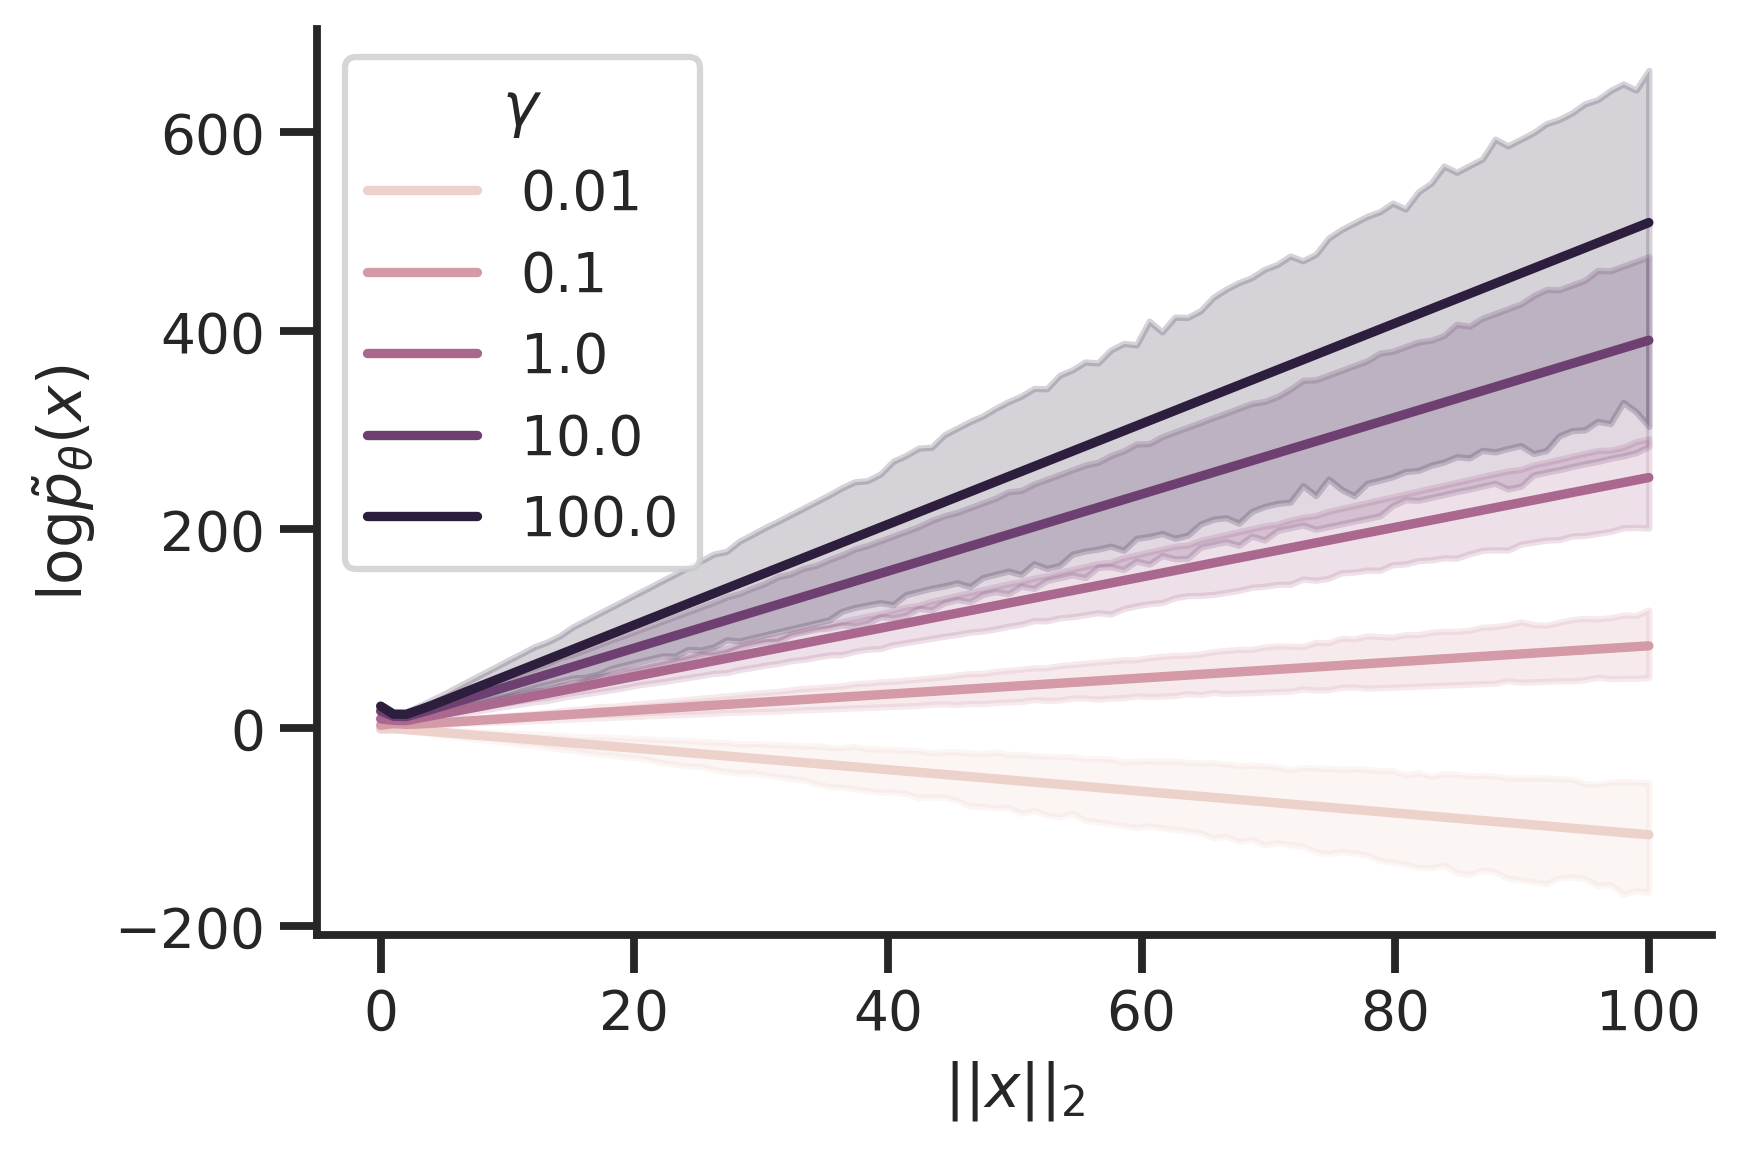
\includegraphics[width=\linewidth]{tables/clf_weight_density_from_training.png}
        }
    \end{center}
    \end{minipage}%
    \hfill
    \begin{minipage}[t]{.48\linewidth}
        \textbf{\small \color{blue}Sidestepping tuning of \(\boldsymbol{\gamma} \)}\\
        Introduce supervision indirectly by training on embeddings obtained from a classification model.
        \begin{center}
        \resizebox{0.5\textwidth}{!}{
        \begin{tabular}{llrr}
\toprule
 Model    & ID dataset &  Natural & Non-natural \\
\midrule
\multirow{2}{*}{CD} & CIFAR-10 &    48.60 &       3.37 \\
     & FMNIST &    95.79 &     -13.52 \\
\midrule
\multirow{2}{*}{SSM} & CIFAR-10 &    53.84 &      -2.31 \\
     & FMNIST &    58.40 &      59.59 \\
\midrule
\multirow{2}{*}{VERA} & CIFAR-10 &    50.16 &      16.97 \\
     & FMNIST &    15.12 &       1.80 \\
\bottomrule
\end{tabular}

        }
        \vspace{0.5em}

        \% improvement in AUC-PR
        \end{center}
        \begin{itemize}
            \item OOD detection significantly improves on \textit{natural} and in cases on \textit{non-natural} datasets
            \item Shows that vanilla \textbf{EBMs struggle to extract high-level, semantic features}
        \end{itemize}

        \vspace{1em}

        \textbf{\color{blue}Can we encourage semantic features?} \\
        Introduce bottlenecks through \(1 \times 1\) convolutions into the architecture.
        \begin{center}
        \resizebox{0.5\textwidth}{!}{
        \begin{tabular}{llrr}
\toprule
 Model    & ID dataset &  Natural &  Non-natural \\
\midrule
\multirow{2}{*}{CD} & CIFAR-10 &    20.18 &        20.38 \\
     & FMNIST &    67.95 &        10.88 \\
\midrule
\multirow{2}{*}{SSM} & CIFAR-10 &    14.76 &        33.34 \\
     & FMNIST &     1.75 &        -5.92 \\
\midrule
\multirow{2}{*}{VERA} & CIFAR-10 &    19.66 &        33.22 \\
     & FMNIST &    26.84 &        32.94 \\
\bottomrule
\end{tabular}

        }
        \vspace{0.5em}

        \% improvement in AUC-PR
        \end{center}
        \vspace{0.45em}

        \begin{itemize}
            \item OOD detection improves consistently upon the baseline EBMs by learning higher-level features
            \item The difference in density assigned for low-level features compared to images increases significantly
        \end{itemize}
        \vspace{1.7em}
        \begin{minipage}[b]{0.5\linewidth}
            \begin{center}
            \resizebox{\textwidth}{!}{
                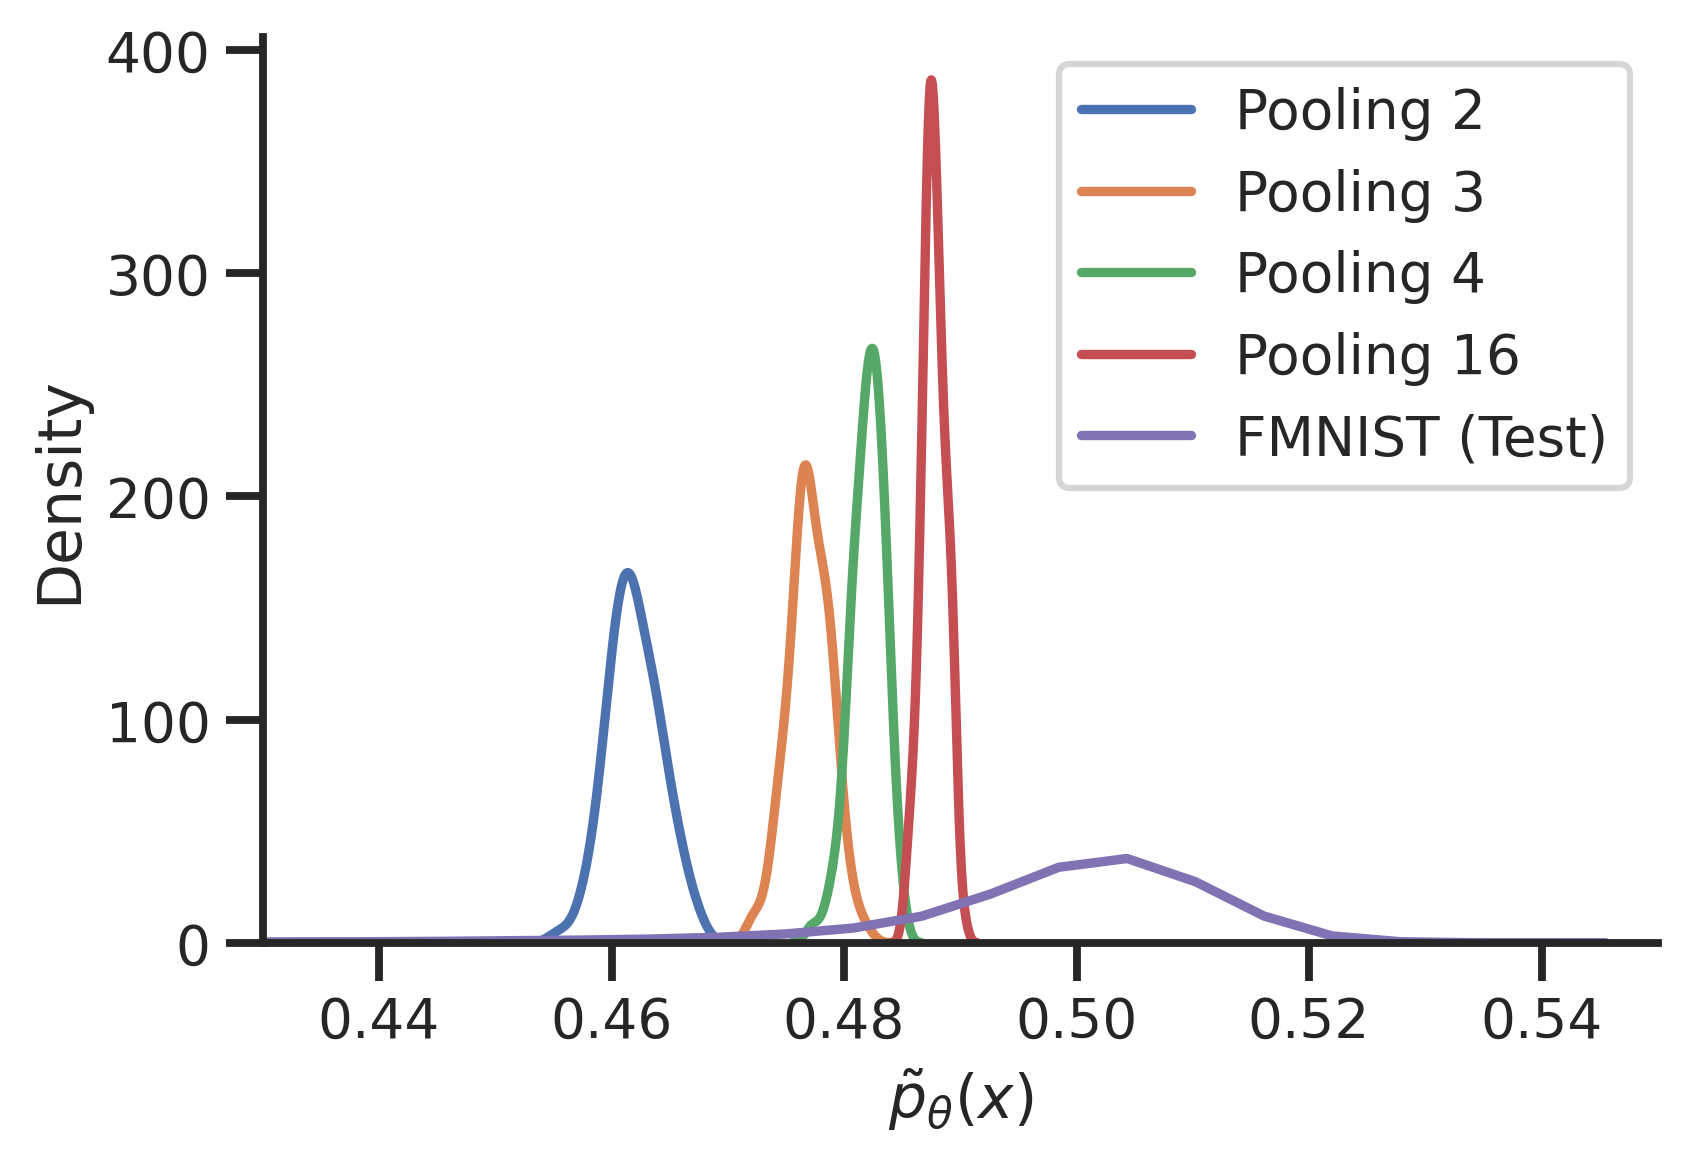
\includegraphics[width=1.1\linewidth]{tables/no_bottleneck_pooling_density_histogram.png}
            }
            No Bottleneck.
            \end{center}
        \end{minipage}%
        \hfill
        \begin{minipage}[b]{0.5\linewidth}
            \begin{center}
            \resizebox{\textwidth}{!}{
                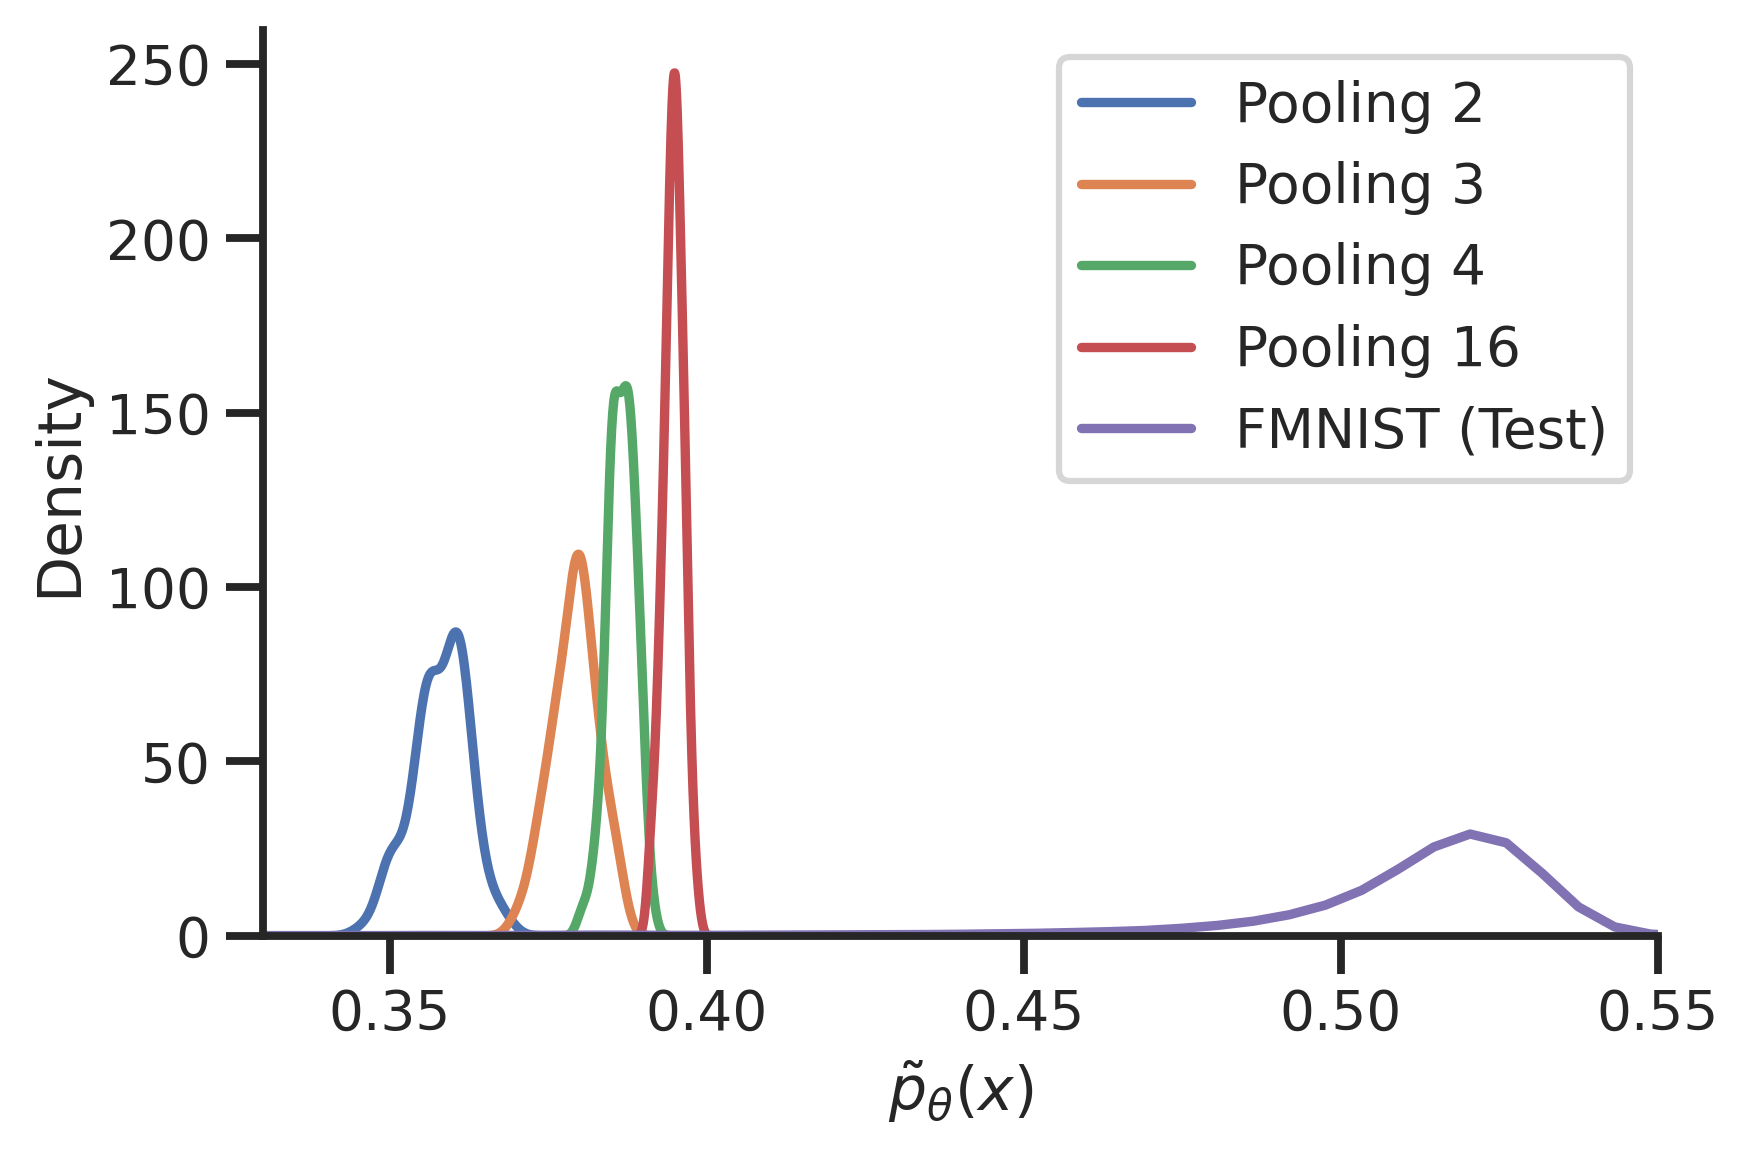
\includegraphics[width=1.1\linewidth]{tables/bottleneck_pooling_density_histogram.png}
            }
            With Bottleneck.
            \end{center}
        \end{minipage}
    \end{minipage}%
    \vspace{-1.5em}
}

%%%%%%%%%%%%%%%%%%%%%%%%%%%%%%%%%%%%%%%%%%%%%%%%%%%%%%%%%%%%%%%%%%%%%%%%%%%%%
\headerbox{\rmfamily What is an energy-based model?}{name=abstract,column=0,below=contribution,span=2}{
    EBM defines a probability distribution over the data \(\mathbf{x} \in \mathbb{R}^D \) through the energy function \( E_\theta \) as

    \begin{equation}
        \label{eq:ebm}
        p_\theta(\mathbf{x}) = \frac{\exp(-E_\theta(\mathbf{x}))}{Z(\theta)}
    \end{equation}

    where \(\smash{Z(\theta) = \int \exp(-E_\theta(\mathbf{x})) d\mathbf{x}}\) is the normalizing constant.% and \(\theta \) are learnable parameters. 
        % In particular, \( E_\theta \) can be any function \( E: \mathbb{R}^D \mapsto \mathbb{R} \) placing no restrictions on the model compared to Normalizing Flows. \\
        %
        % \textbf{Joint Energy model (JEM)~\cite{grathwohlYourClassifierSecretly2020}.}
        % Given a classifier \( f : \mathbb{R}^D \mapsto \mathbb{R}^C \) assigning logits for \(C\) classes for a datapoint \(x \in \mathbb{R}^D\)

        % \begin{equation}
        %     \label{eq:jem_p_y_given_x}
        %     p_\theta(y \mid{} x) = \frac{\exp (f_\theta(x)[y])}{\sum_{y^\prime{}}\exp(f_\theta(x)[y^\prime{}])}
        % \end{equation}

        % where \( f_\theta(x)[y] \) denotes the \(y \)-th logit.
        % %
        % The logits \( f_\theta(x)[y] \) can be interpret as unnormalized probabilities of the joint distribution \(p_\theta(x, y) \)
        % %
        % % \begin{equation}
        % %     p_\theta(x, y) = \frac{\exp(f(x)[y])}{Z_\theta}
        % % \end{equation}
        % which yields the marginal distribution over \(x\) as

        % \begin{equation}
        %     \label{eq:jem_p_x}
        %     p_\theta(x) = \sum_y p_\theta (x, y) = \sum_y \frac{\exp(f(x)[y])}{Z(\theta)}
        % \end{equation}
        % \textbf{Training.}
        % We follow~\cite{grathwohlYourClassifierSecretly2020} and optimize the factorization 
        % %
        % \begin{equation}
        %     \log p_\theta(x, y) =  \log p_\theta(x) + \log p_\theta(y \mid x)
        % \end{equation}
        % %
        % using~\ref{eq:jem_p_y_given_x} and~\ref{eq:jem_p_x}. In particular, we use a Cross Entropy objective to optimize \(\smash{p_\theta(y \mid x)}\) weighted with hyperparameter \(\gamma \). \\
        %
    \vspace{1em}
    {\bf\color{blue} Properties:}

    \makebox[0.01\textwidth]{} 
    \begin{minipage}[t]{0.44\textwidth}
        \begin{itemize}
            \item[\cmark{}] Flexible transformations
            \item[\cmark{}] Dimensionality reduction
        \end{itemize}
    \end{minipage}%
    \begin{minipage}[t]{0.46\textwidth}
        \begin{itemize}
            \item[\xmark{}] Exact density evaluation
            \item[\xmark{}] No direct maximum likelihood training
        \end{itemize}
    \end{minipage}
}

\headerbox{\rmfamily Why study EBMs for OOD detection?}{name=motivation,column=0,below=abstract,span=2}{
    \begin{itemize}
        \item Recent research on generative models for OOD detection focuses on exact likelihood methods, e.g., Normalizing Flows \\
        \(\rightarrow \) We compare behavior for EBMs vs. Normalizing Flows
        \item EBMs show good OOD detection capabilities~\cite{grathwohlYourClassifierSecretly2020}, however, no detailed analysis has been done \\
        \(\rightarrow \) We consider EBMs trained with different approaches \\
        \(\rightarrow \) We investigate influences like supervision, dimensionality reduction, and architecture
    \end{itemize} 

    % \vspace{1em}
    % {\bf\color{blue} \(\rightarrow \) Hypotheses for better OOD detection vs. Normalizing Flows:}
    % \begin{itemize}
    %     \item \textbf{Dimensionality reduction}: Normalizing Flows operate in original data space, 
    %     \item Supervision: JEMs \cite{grathwohlYourClassifierSecretly2020} introduce supervision into EBMs, while it is not considered for Normalizing Flows.
    %}\end{itemize}

    %\begin{center}
    %\begin{tabular}{lll}
    %                        & \textbf{Normalizing Flows}              & \textbf{EBM}                  \\
    %\midrule
    %\textbf{Dimensionality reduction} & Operate in \(\mathbb{R}^D\) &  \(E_\theta : \mathbb{R}^D \mapsto \mathbb{R}\) \\
    %\textbf{Supervision}              & Not considered                 & Used in JEM~\cite{grathwohlYourClassifierSecretly2020}         
    %\end{tabular}%
    %\end{center}
}

\headerbox{\rmfamily How to train an EBM?}{name=training,column=0,below=motivation,span=2}{
    We consider three approaches to train EBMs.
    
    \vspace{0.5em}

    \textbf{\color{blue} Sliced score matching (SSM)~\cite{songSlicedScoreMatching2019}.}
    Efficient update formula based on random projection
    
    \begin{equation}
        \mathbb{E}_{p_\mathbf{v}} \mathbb{E}_{p(\mathbf{x})} \left[\mathbf{v}^T \nabla_\mathbf{x} s_\theta(\mathbf{x})\mathbf{v} + \frac{1}{2} \lVert s_\theta(\mathbf{x}) \rVert^2_2 \right] \nonumber
    \end{equation}

    where \(s_\theta(\mathbf{x}) = \nabla_\mathbf{x} p_\theta(\mathbf{x})\) and \(\mathbf{v} \sim p_\mathbf{v}\) is a simple distribution of random vectors. \\
    %
    
    \vspace{0.5em}

    \textbf{\color{blue} Contrastive divergence (CD)~\cite{hintonTrainingProductsExperts2002}.}
    Approximation of the gradient of the maximum likelihood objective by
    %
    \begin{equation}
    \label{eq:cd}
        \nabla_\theta p_\theta(\mathbf{x}) = \mathbb{E}_{p_\theta(\mathbf{x}^\prime)} \left[ \nabla_\theta E_\theta(\mathbf{x}^\prime) \right] - \nabla_\theta E_\theta(\mathbf{x}) \nonumber
    \end{equation}
    %
    
    \vspace{0.5em}

    \textbf{\color{blue}VERA~\cite{grathwohlNoMCMCMe2020}.}
    Learn the parameters \(\phi \) of a auxiliary distribution \(q_\phi \) as the optimum of
    %
    \begin{equation}
        \log Z(\theta) = \max_{q_\phi} \mathbb{E}_{q_\phi(\mathbf{x})} \left[ f_\theta(\mathbf{x}) \right] + H(q_\phi) \nonumber
    \end{equation}
    %
    which can be plugged into Eq. (1) to obtain an alternative method for training EBMs with a variational approximation to estimate the entropy term \(H(q_\phi)\).\\
}

\headerbox{\rmfamily References}{name=references,column=2,below=results,span=3}{
    \footnotesize{
    \bibliography{paper}
    }
}


\end{poster}
\end{document}
